\section{\label{sec:simulation}Simulation using \ES{}}

\subsection{Setting up \ES{}}

Electrokinetics is a relatively new feature of \ES{} and new functionality is still being added. This is why it is advisable to get a copy of the current \ES{} master to work with. If you don't already have a working copy of the \ES{} master, follow tutorial \texttt{00-building\_espresso}. Enable the features \texttt{ELETROKINETICS} and \texttt{EK\_BOUNDARIES} during the build process.

\subsection{\label{sec:units}Mapping SI and Simulation Units}

\ES{} does not predefine any unit system. This makes it more flexible but also requires us to spend some thought on the conversion from SI units to simulation units and back. Since most first time users have trouble with this, we will go through that process in detail here.
	
Important to note is that \ES{}'s unit system is nothing more than a rescaled variant of the SI system. All physical formulas you are used to in the SI system remain valid and you can use them to find relations between your units. Lets start by choosing a unit of length. Since we are going to deal with Debye layers with extensions of nanometers, a sensible choice is
%
\begin{align*}
[x]=1\U{nm}.
\end{align*}
%
The involved energies are of the magnitude of $\kT$. We will simulate our system at room temperature ($300\U K$), hence we use as unit of energy
\begin{align*}
[E]=k_B\cdot300\U K\approx4.14\E{-21}\U J.
\end{align*}
%
By default ESPResSo has no concept for particle masses (but the feature can be activated). That means all particle masses are assumed to be $1\,[\mathrm{m}]$, which forces us to use the particle mass as mass unit. For this simulation we use the mass of sodium ions, which is
\begin{align*}
[m]=23\U u\approx3.82\E{-26}\U{kg}.
\end{align*}
%
For the relation
\begin{align*}
E=\frac 1 2 mv^2
\end{align*}
%
to hold, the unit of time has to be defined so that
\begin{align*}
[E]=[m]\cdot\frac{[x]^2}{[t]^2}.
\end{align*}
%
From that we get the missing unit of time
\begin{align*}
[t]=[x]\cdot\sqrt{\frac{[m]}{[E]}}=1\U{nm}\cdot\sqrt{\frac{23\U u}{k_B\cdot 300\U K}}\approx 3.03760648\E{-12}\U s\approx3.04\U{ps}.
\end{align*}
%
The last unit we need is the one of charge. We choose it to be the elementary charge
\begin{align*}
[q]=e\approx1.60\E{-19}\U C.
\end{align*}
%
We now have all the units necessary to convert out simulation parameters.

\begin{tabular}[h]{|l|c|c|}
\hline
parameter & value (SI units) & value (simuation units)\\
\hline\hline
channel width $d$ & $50\U{nm}$ & $50\U{[x]}$\\
\hline
thermal energy $k_B T$ & $k_B\cdot300\U K$ & $1\U{[E]}$\\
\hline
Bjerrum length $l_B$ & $0.7095\U{nm}$ & $0.7095\U{[x]}$\\
\hline
counterion charge $q$ & $1e$ & $1\U{[q]}$\\
\hline
counterion diffusion coefficient $D$ & $2.0\E{-9}\U{m^2/s}$ & $0.006075\U{[x]^2/[t]}$\\
\hline
solvent density $\rho$ & $1.0\E{3}\U{kg/m^3}$ & $26.18\U{[m]/[x]^3}$\\
\hline
kinematic solvent viscosity $\eta$ & $1.0\E{-3}\U{Pa}\U{s}$ & $79.53\U{[m]/([x][t])}$\\
\hline
external electrical field $E$ & $2.585\E{6}\U{V/m}$ & $0.1\U{[E]/[q][x]}$\\
\hline
\end{tabular}
\\

ESPResSo determines the strength of the electrostatic interactions via the Bjerrum-length $l_B$. That is the length for which the electrostatic interaction energy of two elementary charges equals the thermal energy
%
\begin{align*}
k_B T=\frac{e^2}{4\pi\varepsilon_0\varepsilon_r}\cdot\frac 1 {l_B}.
\end{align*}
%
For water at $300\U{K}$ with $\varepsilon_r = 78.54$ it is $l_B\approx0.7095\U{nm}$.


\subsection{Setting up the slip pore system}

The script for this simulation comes with this tutorial and is called \texttt{eof\_electrokinetics.tcl}. All used commands are documented in the User's Guide in the section called ``Electrokinetics''.

We first set up a periodic simulation box of the desired dimensions. Note that the dimensions are of course given in simulation units.

\begin{lstlisting}
# Set the slit pore geometry the width is the non-periodic part of the geometry
# the padding is used to ensure that there is no field outside the slit

set box_x 6
set box_y 6
set width 50

set padding 6
set box_z [expr $width+2*$padding]

setmd box_l $box_x $box_y $box_z
\end{lstlisting}

We then store all the parameters we calculated in section~\ref{sec:units}. At this point, these parameters only reside in TCL variables. They will only be used by \ES{} once they are being passed to the respective initialization functions.

\begin{lstlisting}[firstnumber=13]
# Set the electrokinetic parameters

set agrid 1.0
set dt 0.2
set kT 1.0
set bjerrum_length 0.7095
set D 0.006075
set valency 1.0
set viscosity_dynamic 79.53
set density_water 26.15
set sigma -0.05
set ext_force 0.1
\end{lstlisting}

Before we initialize the actual electrokinetics algorithm, we need to set the time step and some other parameters that are not actually used, but would otherwise lead to error messages.

\begin{lstlisting}[firstnumber=26]
# Set the simulation parameters

setmd time_step $dt
setmd skin 0.1
thermostat off
set integration_length 200000
\end{lstlisting}

We can now initialize the electrokinetics algorithm. All functionality pertaining to this algorithm is available through the \texttt{electrkinetics} command. Please note that the fluid viscosity is specified as a kinematic viscosity, which is the dunamic viscosity divided by the fluid density. The kinematic viscosity is also required if you initialize the pure lattice-Boltzmann method.

\begin{lstlisting}[firstnumber=33]
# Set up the (LB) electrokinetics fluid

set viscosity_kinematic [expr $viscosity_dynamic/$density_water]
electrokinetics agrid $agrid lb_density $density_water viscosity $viscosity_kinematic friction 1.0 T $kT bjerrum_length $bjerrum_length
\end{lstlisting}

The friction parameter in the previous initialization command is again not used but needs to be specified to pass the sanity check of the LB.

Next, we initialize the individual ionic species. In this case, we only set up one species of positively charged counterions. The integer coming after the \texttt{electrkinetics} command denotes the species. Future commands issued with this number will change the species properties. The species' numbers do not have to be issued in succession.

\begin{lstlisting}[firstnumber=38]
# Set up the charged and neutral species

set density_counterions [expr -2.0*double($sigma)/double($width)]
electrokinetics 1 density $density_counterions D $D valency $valency ext_force $ext_force 0 0
\end{lstlisting}

The \texttt{electrokinetics boundary} command takes the keyword \texttt{charge\_density} and the numerical charge density in simulation units as the first two arguments. The syntax for the remaining arguments is the same as for the \texttt{lbboundary} command. Here we initialize two sets of boundaries. For each of the two sides a rhomboid shaped charged slice and an uncharged wall covering the whole padding region.

\begin{lstlisting}[firstnumber=43]
# Set up the charged boundaries

electrokinetics boundary charge_density [expr $sigma/$agrid] rhomboid corner 0 0 [expr $padding-$agrid] c 0 0 $agrid b $box_x 0 0 a 0 $box_y 0 direction outside
electrokinetics boundary charge_density [expr $sigma/$agrid] rhomboid corner 0 0 [expr $padding+$width] c 0 0 $agrid b $box_x 0 0 a 0 $box_y 0 direction outside

# Set up the walls confining the fluid

electrokinetics boundary charge_density 0.0 wall normal 0 0 1 d $padding 0 0 direction outside
electrokinetics boundary charge_density 0.0 wall normal 0 0 -1 d -[expr $padding+$width] 0 0 direction outside
\end{lstlisting}

After setting up the system, we integrate a sufficient number of time steps to relax the system into the stationary state and output the counterion density profile, the velocity profile, and the shear stress. Since this system has translational symmetry in the x- and y-direction, we iterate over a line in the z direction and use the \texttt{electrokinetics node} command, to output local quantities. You can instead also use the \texttt{electrokinetics print} command to output the whole field at once in a Paraview compatible format.

Density and velocity are not the only fields available for output. Please refer to the User's Guide for all available options.

\begin{lstlisting}[firstnumber=53]
# Integrate the system

integrate $integration_length

# Output

set fp [open "eof_electrokinetics.dat" "w"]
puts $fp "#position measured_density measured_velocity measured_pressure_xz"

for {set i 0} {$i < [expr $box_z/$agrid]} {incr i} {
  if {[expr $i*$agrid] >= $padding && [expr $i*$agrid] < [expr $box_z - $padding] } {
    set xvalue [expr $i*$agrid - $padding]
    set position [expr $i*$agrid - $padding - $width/2.0 + $agrid/2.0]

    # density
    set measured_density [electrokinetics 1 node [expr int($box_x/(2*$agrid))] [expr int($box_y/(2*$agrid))] $i print density]

    # velocity
    set measured_velocity [lindex [electrokinetics node [expr int($box_x/(2*$agrid))] [expr int($box_y/(2*$agrid))] $i print velocity] 0]

    # xz component pressure tensor
    set measured_pressure_xz [lindex [lbnode [expr int($box_x/(2*$agrid))] [expr int($box_y/(2*$agrid))] $i print pi_neq] 3]

    puts $fp "$position $measured_density $measured_velocity $measured_pressure_xz"
  }
}

close $fp
\end{lstlisting}

With this tutorial also came a Gnuplot script \texttt{plot.gp}. If everything went well, running this script with Gnuplot from a folder containing the output files \texttt{eof\_analytical.dat} and \texttt{eof\_electrokinetics.dat} should produce the result shown in Figure~\ref{fig:result}.

\begin{figure}[h]
  \begin{center}
  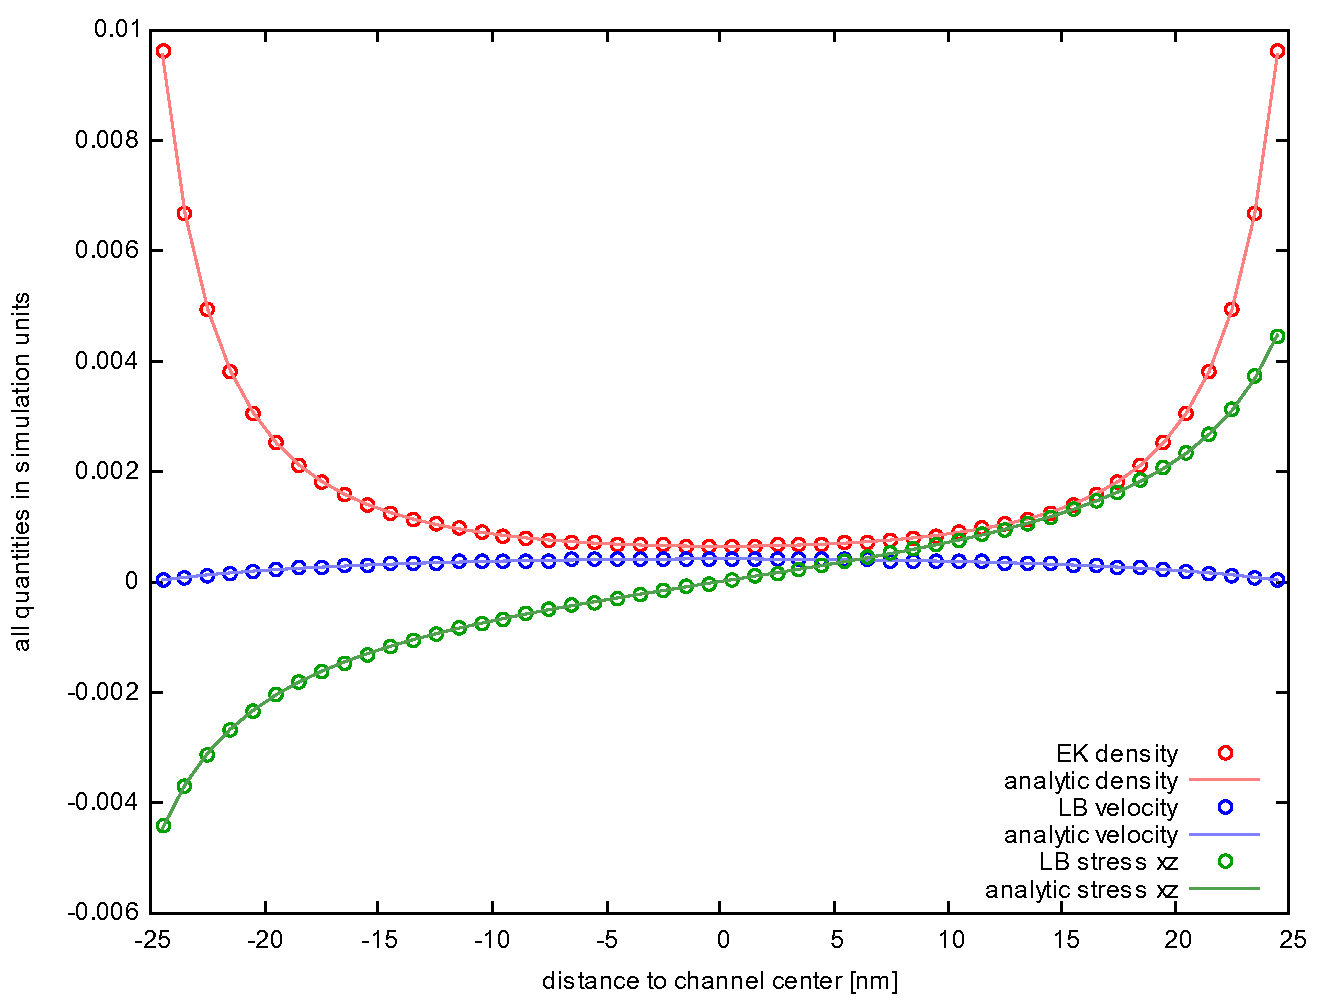
\includegraphics[width=1.0\columnwidth]{figures/profiles.pdf}
  \end{center}
  \caption{\label{fig:result}Profiles along the direction perpendicular to the slit pore walls for the counterion density, fluid velocity, and fluid shear stress. Parameters as chosen in Section~\ref{sec:units}.}
\end{figure}
